%%%%%%%%%%%%%%%%%%%%%%%%%%%%%%%%%%%%%%%%%%%%%%%%%%%%%%%%%%%%%%%%%%%%%
% LaTeX Template: Project Titlepage Modified (v 0.1) by rcx
%
% Original Source: http://www.howtotex.com
% Date: February 2014
% 
% This is a title page template which be used for articles & reports.
% 
% This is the modified version of the original Latex template from
% aforementioned website.
% 
%%%%%%%%%%%%%%%%%%%%%%%%%%%%%%%%%%%%%%%%%%%%%%%%%%%%%%%%%%%%%%%%%%%%%%

\documentclass[12pt]{report}
\usepackage[a4paper]{geometry}
\usepackage[myheadings]{fullpage}
\usepackage{fancyhdr}
\usepackage{lastpage}
\usepackage{graphicx, wrapfig,setspace, booktabs}
\usepackage[T1]{fontenc}
\usepackage[font=small, labelfont=bf]{caption}
\usepackage{fourier}
\usepackage[protrusion=true, expansion=true]{microtype}
\usepackage[english]{babel}
\usepackage{sectsty}
\usepackage{lipsum}
\usepackage[hyphens]{url}
\usepackage{subfig}
\usepackage{alphalph}
\renewcommand*{\thesubfigure}{%
\alphalph{\value{subfigure}}%
}%


\newcommand{\HRule}[1]{\rule{\linewidth}{#1}}
\onehalfspacing
\setcounter{tocdepth}{5}
\setcounter{secnumdepth}{5}
\usepackage{float}
%-------------------------------------------------------------------------------
% HEADER & FOOTER
%-------------------------------------------------------------------------------
\pagestyle{fancy}
\fancyhf{}
\setlength\headheight{15pt}
\fancyhead[L]{CS4011: Contest}
\fancyhead[R]{Machine Learning}
\fancyfoot[R]{Page \thepage\ of \pageref{LastPage}}
%-------------------------------------------------------------------------------
% TITLE PAGE
%-------------------------------------------------------------------------------

\begin{document}

\title{ \normalsize \textsc{CS4011 : Introduction to Machine Learning}
		\\ [2.0cm]
		\HRule{0.5pt} \\
		\LARGE \textbf{\uppercase{Report}}
		\HRule{2pt} \\ [0.5cm]
		\normalsize \today \vspace*{5\baselineskip}}

\date{}

\author{
		Student ID: EE15B123 ${\&}$ EE15B025 \\ 
		Namida M \\
		Ganga Meghanath }

\renewcommand\thesection{\arabic{section}}
\maketitle
\tableofcontents
\newpage

%-------------------------------------------------------------------------------
% Section title formatting
\sectionfont{\scshape}
%-------------------------------------------------------------------------------

%-------------------------------------------------------------------------------
% BODY
%-------------------------------------------------------------------------------

\section{Introduction}
Machine learning is a type of artificial intelligence (AI) that allows software applications to become more accurate in predicting outcomes without being explicitly programmed. The basic premise of machine learning is to build algorithms that can receive input data and use statistical analysis to predict an output value within an acceptable range. \\

Machine learning algorithms are often categorized as being supervised or unsupervised. Supervised algorithms require humans to provide both input and desired output, in addition to furnishing feedback about the accuracy of predictions during training. Once training is complete, the algorithm will apply what was learned to new data. Unsupervised algorithms do not need to be trained with desired outcome data. Instead, they use an iterative approach called deep learning to review data and arrive at conclusions.

\section{Folder Structure}
\graphicspath{ {Images/} }
\begin{figure}[H]
  \centering
  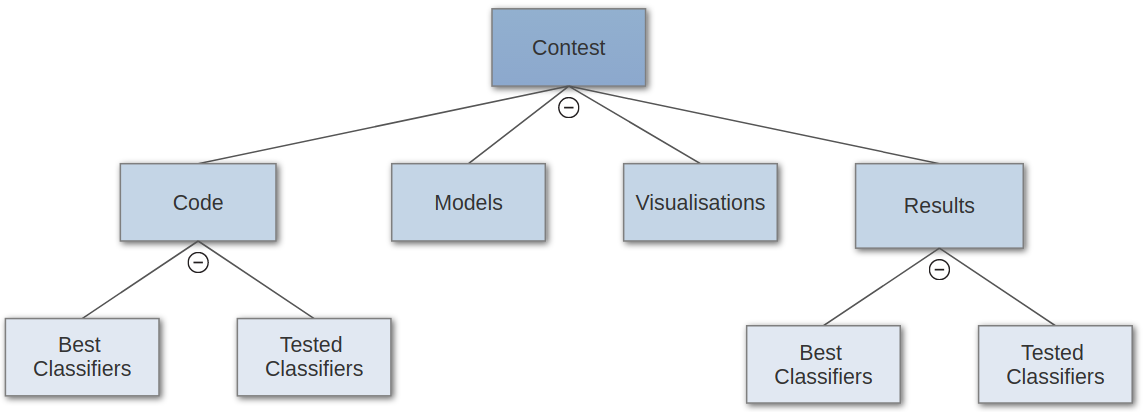
\includegraphics[width=1\textwidth]{Images/flow_chart.png}\label{fig:f1}
\end{figure}


%-------------------------------------------------------------------------------
%DATA ANALYSIS
%-------------------------------------------------------------------------------
\newpage
\section{Data Analysis}
\subsection{General observations}
We have been given a dataset consisting of 29 classes with 9501 training instances, of dimension 2600. The class based distribution has been shown below.

\graphicspath{ {Images/} }
\begin{figure}[H]
  \centering
  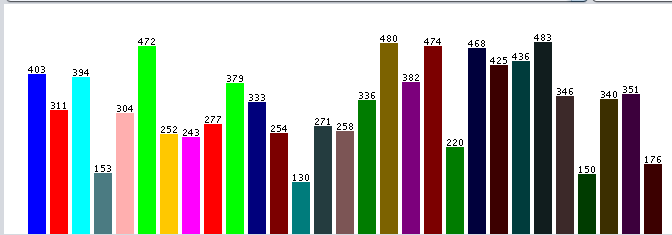
\includegraphics[width=1\textwidth]{class_distribution.png}\label{fig:f1}
  \caption{Class Distribution}
\end{figure}

\begin{figure}[H]
  \centering
  \subfloat[f1405 vs f2368]{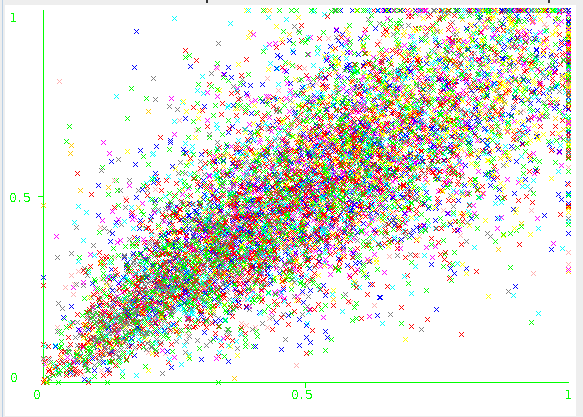
\includegraphics[width=0.4\textwidth]{c_1405_2368.png}}
  \hfill
  \subfloat[f1371 vs f2433]{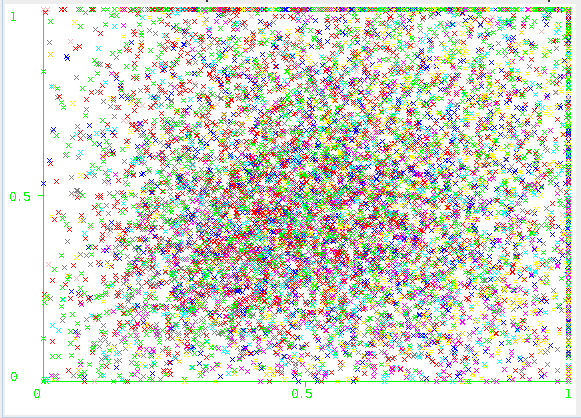
\includegraphics[width=0.4\textwidth]{c_f_1371_2433.png}}
  \vfill
  \subfloat[f681 vs f2564]{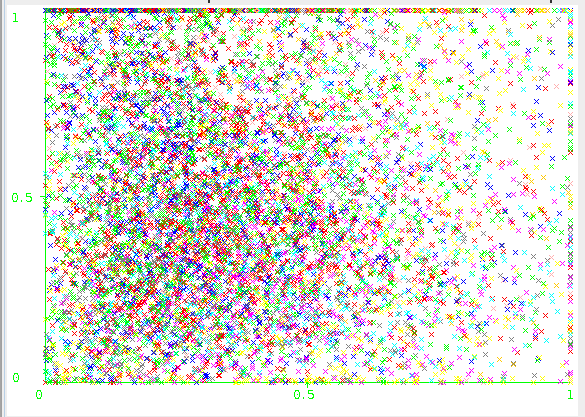
\includegraphics[width=0.4\textwidth]{c_f_681_2546.png}}
  \hfill
  \subfloat[f697 vs f2571]{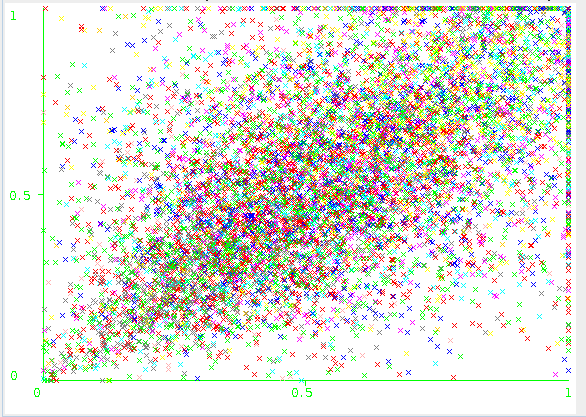
\includegraphics[width=0.4\textwidth]{c_f_697_2571.png}}
\end{figure}

\begin{figure}[H]
  \centering
  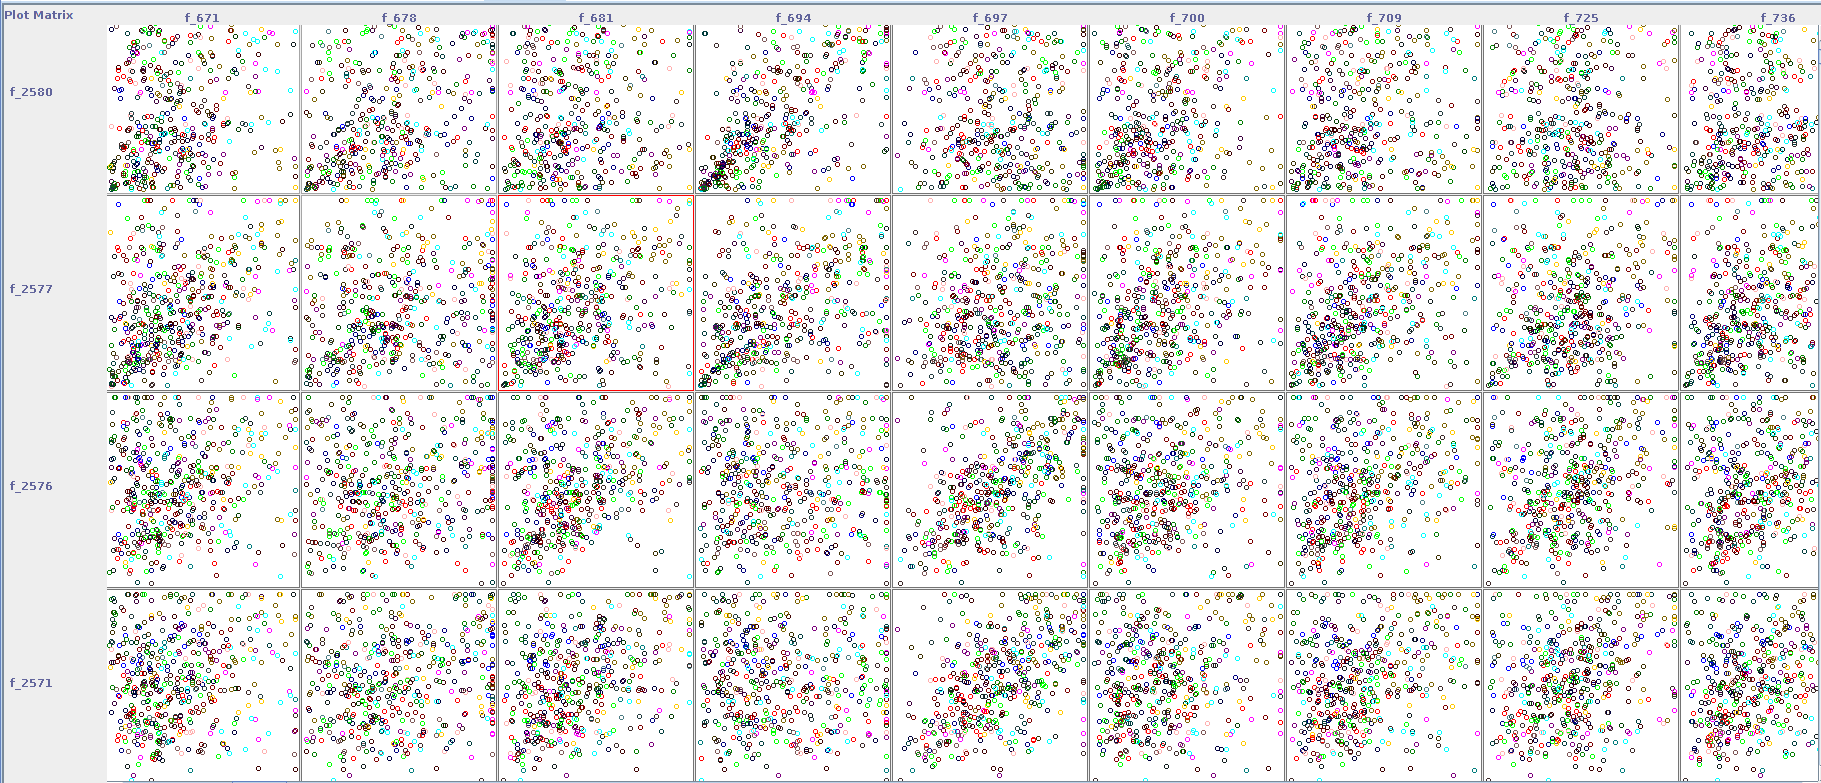
\includegraphics[width=1\textwidth]{Matrix2.png}
  \caption{Feature Analysis}
\end{figure}

\begin{figure}[H]
  \centering
  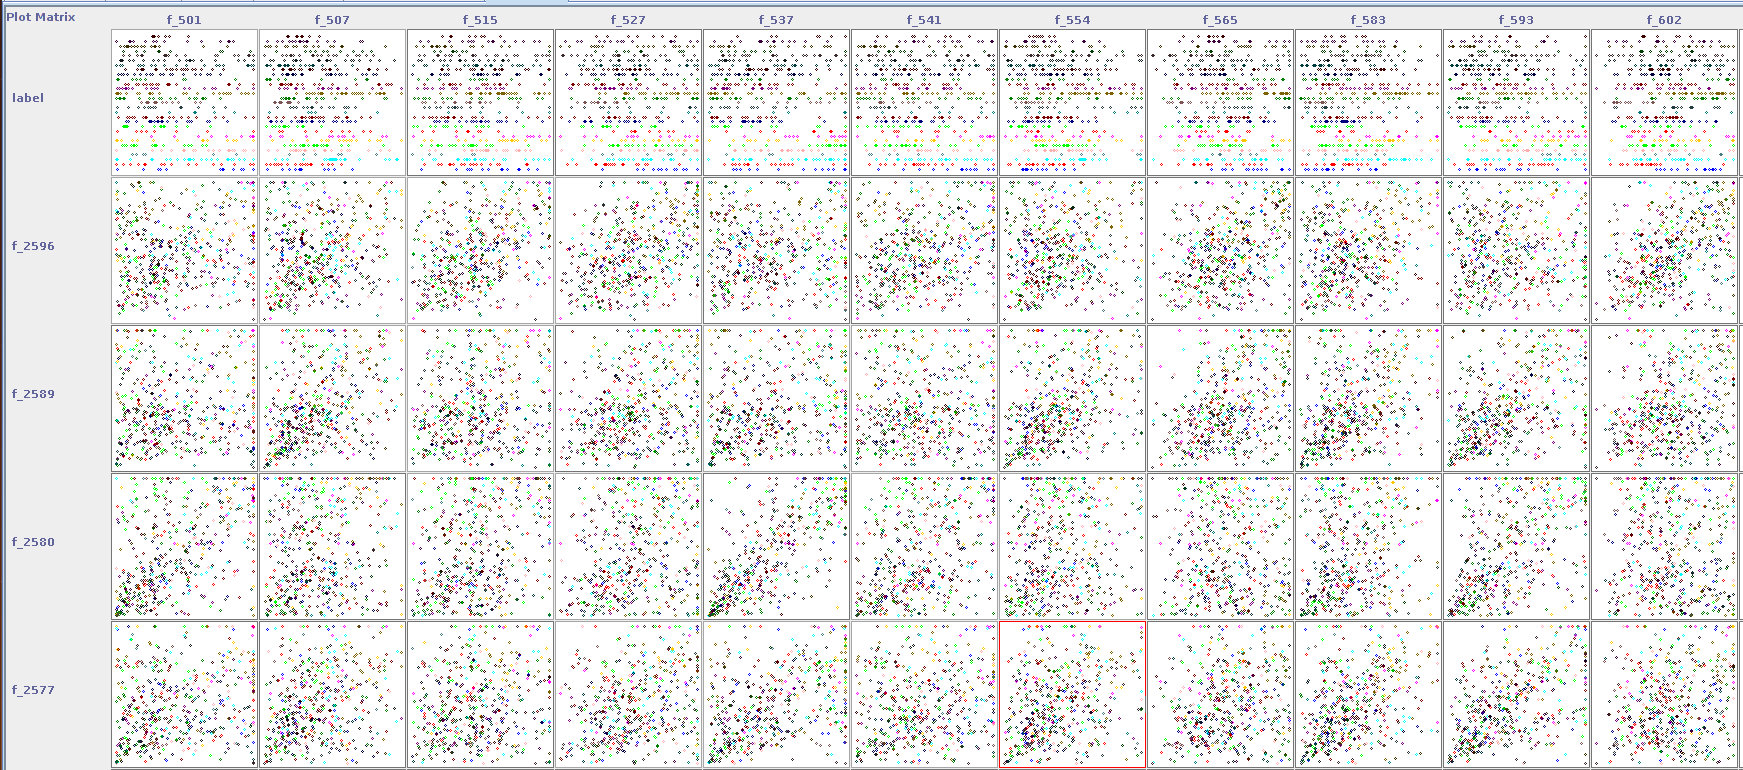
\includegraphics[width=1\textwidth]{matrix1.png}
  \caption{Feature Analysis}
\end{figure}

We can observe from the figures that there are correlated features in the data. Hence, we can try out different dimensionality techniques on the data to reduce the feature space. This will help reduce the computation time, as well as remove unwanted features from the dataset.\\ 

Also, it is likely that there is a lot of overlap between the different classes in the original 2600 dimensional space. Hence, the classification task is probably difficult. This can be infered from the above figures upon seeing the scattered data.\\

The initial figure also gives us understanding about the class imbalance that exists in the provided dataset that might make recognition of minority class instances difficult.\\

The class-based distribution of data along some features have been depicted below :

\begin{figure}[H]
  \centering
  \subfloat[f997]{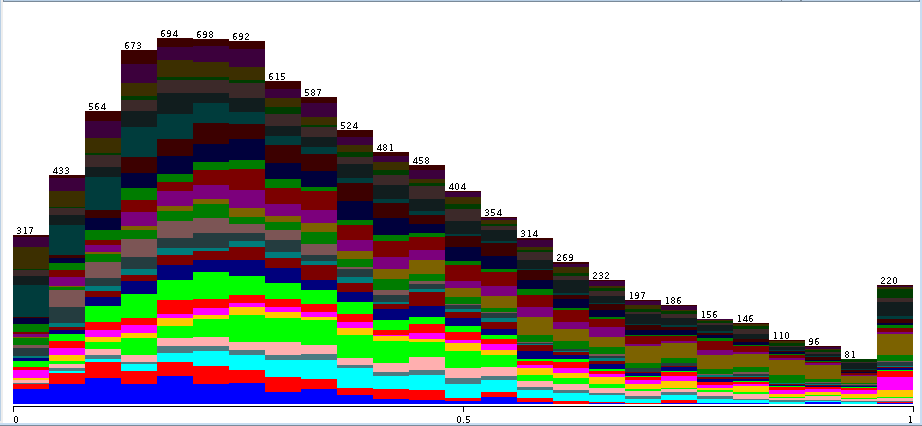
\includegraphics[width=0.45\textwidth]{997.png}}
  \hfill
  \subfloat[f1663]{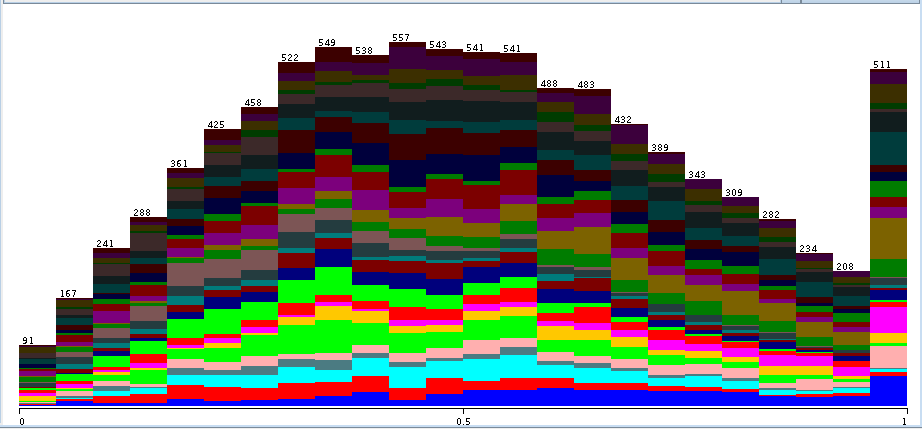
\includegraphics[width=0.45\textwidth]{f_1663.png}}
  \vfill
  \subfloat[f2033]{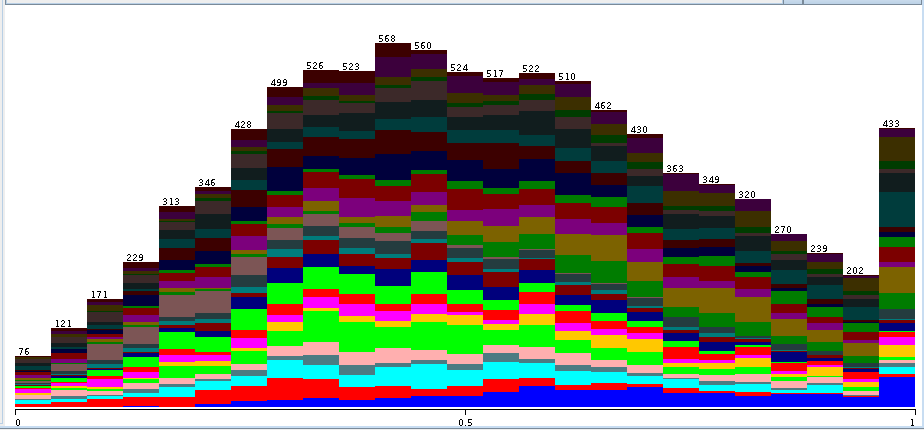
\includegraphics[width=0.45\textwidth]{f_2033.png}}
  \hfill
  \subfloat[f2546]{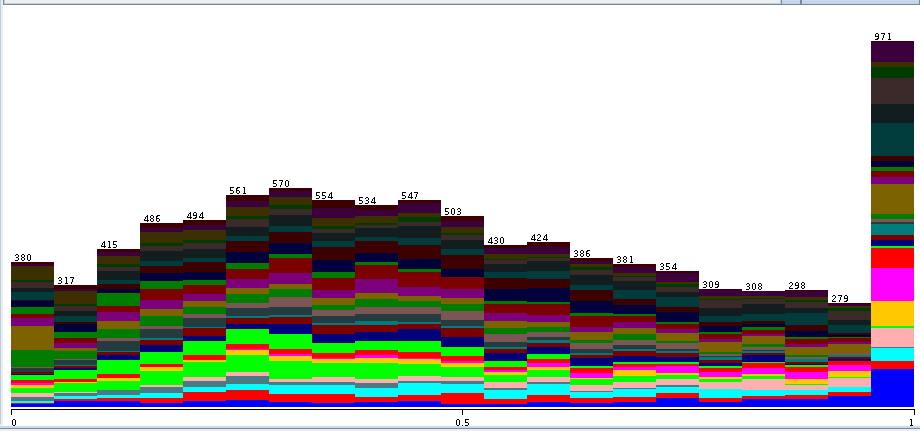
\includegraphics[width=0.45\textwidth]{f_2546.png}}
  \vfill
  \subfloat[f507]{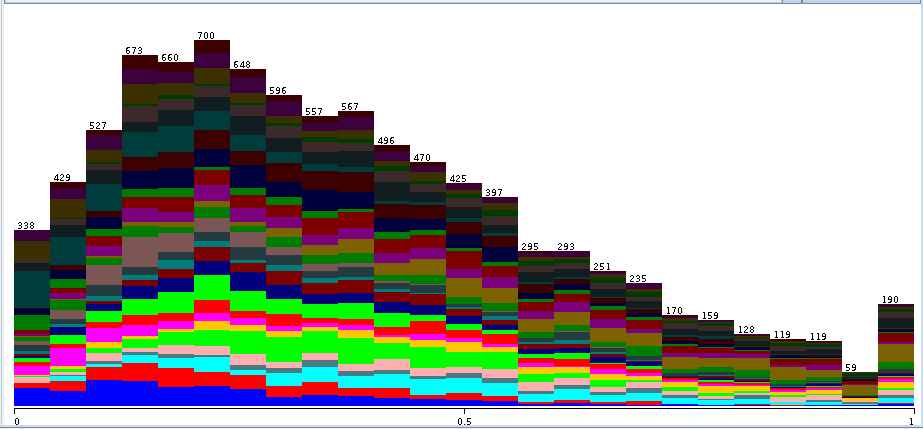
\includegraphics[width=0.45\textwidth]{f_507.png}}
  \hfill
  \subfloat[f996]{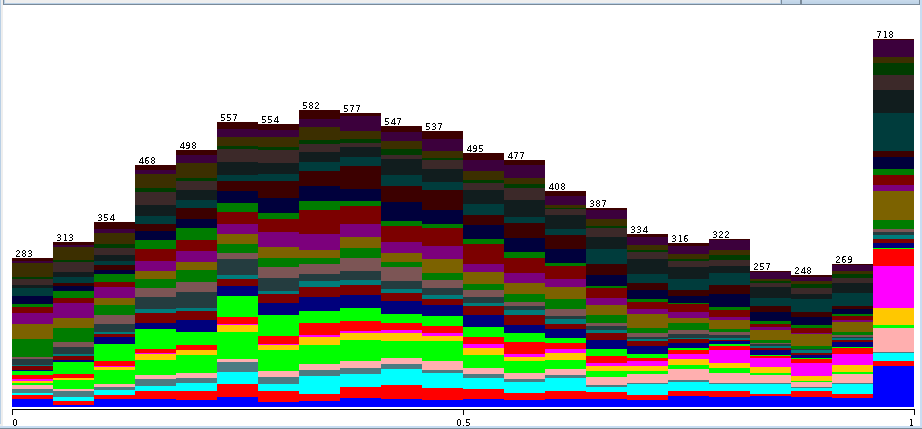
\includegraphics[width=0.45\textwidth]{f_996.png}}
\end{figure}

\subsection{Missing Value Analysis}
In real world data, many a times, one is not able to get values for all features of a data point. Depending on the number of missing values, and the pattern in which they are missing, the imputation strategy becomes really important.\\

The statistics of the missing values in the given dataset are as follows :

\begin{table}[H]
\label{T:equipos}
\begin{center}
\begin{tabular}{| c | c |}
\hline
\textbf{View} & \textbf{Estimates of regions missing values}\\
\hline

Datapoints & Average of 200 in each row  \\ \hline
Features & Around 3750 in each of the first 500 columns \\ \hline

\end{tabular}
\end{center}
\end{table}

The frequency plots are as follows :

\begin{figure}[H]
  \centering
  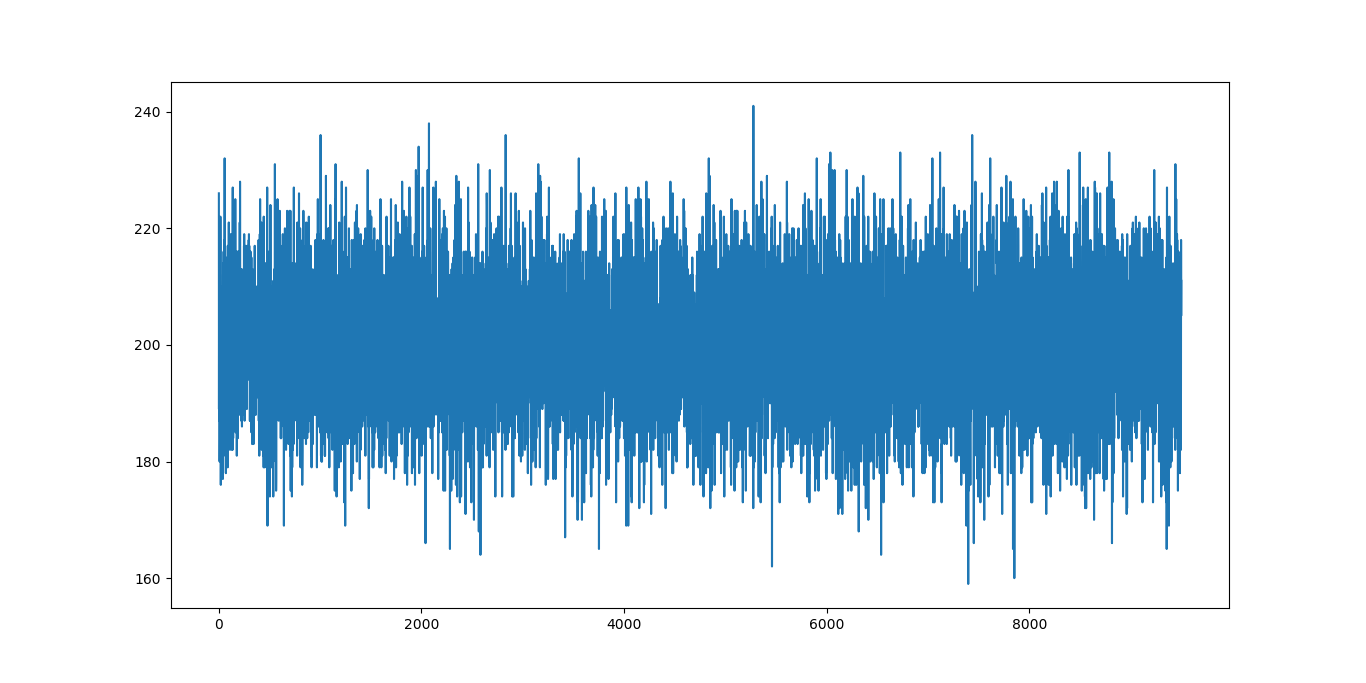
\includegraphics[width=1\textwidth]{row_wise.png}
  \caption{Train data: Plot of no. of missing attributes vs each datapoint}
\end{figure}


\begin{figure}[H]
  \centering
  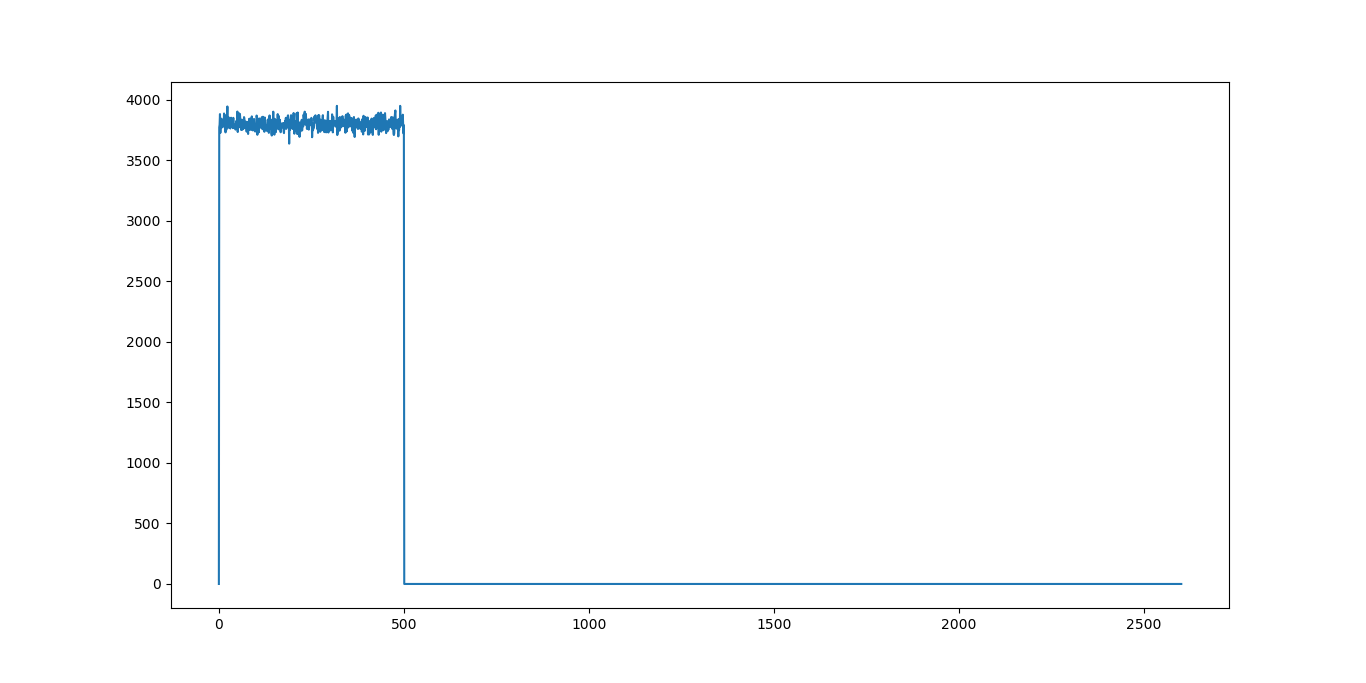
\includegraphics[width=1\textwidth]{col-wise.png}
  \caption{Train-data: Plot of no. of missing values vs attribute index}
\end{figure}


\begin{figure}[H]
  \centering
  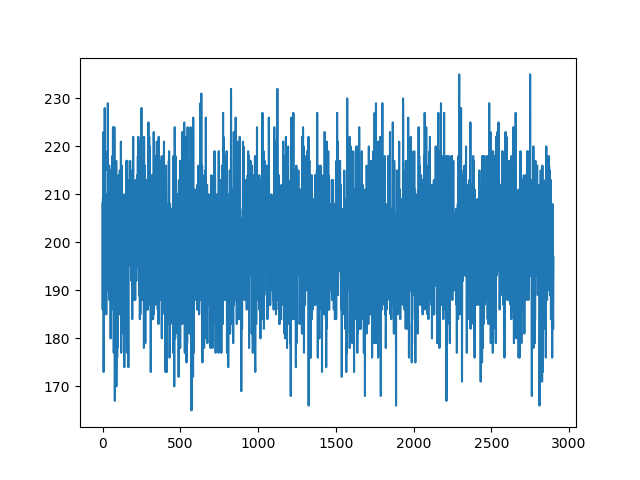
\includegraphics[width=0.8\textwidth]{row_wise_test.png}
  \caption{Test-data: Plot of no. of missing values vs attribute index}
\end{figure}

\begin{figure}[H]
  \centering
  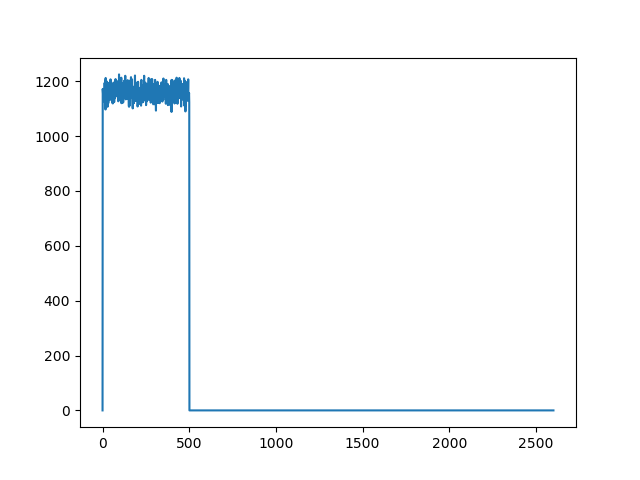
\includegraphics[width=0.8\textwidth]{col_wise_test.png}
  \caption{Test-Data: Plot of no. of missing values vs data point}
\end{figure}


\subsection{Imputation and Removal}
There are four simple options we can use in such cases:
\begin{itemize}
  \item Mean Imputation \\
  Advantage -  mean of each feature is preserved.\\
  Disadvantage - same value inserted in all vacancies in a column. Hence when the statistics of missing values per column is high, the contribution of the column towards class prediction decreases significantly (especially if the missing values have roughly equal in number for each class (or weighted by no. of instances in each class) 
  \item Median Imputation: 
  Advantage:The median value is mostly unaffected by outliers.
  \item Mode Imputation
  \item Remove rows/columns: In cases where there are too many values missing to make any proper inferences about the data, it may be best to not use the data at all. Even if we use regression to fill in values , the feature itself may become redundant. 
  
\end{itemize}

Other possible ways :
\begin{itemize}
    \item Linear Regression : Initial 500 attributes in the given dataset have missing values. Hence linear regression models are built using the rest of the 1500 attributes to predict the missing values in the first 500 attributes. This is by assuming that the attributes consisting of missing can be roughly represented as some linear combination of the last 1500 attributes.
    \item Correlation : Replacing the missing values using another attribute that is highly correlated with the attribute consisting of missing values.
    \item Class-conditioned Regression : Consider the class as an attribute during linear regression or do class-wise linear regression, ie, linear regression for each class separately. But this cannot be implemented on the test data since class labels are not available. Hence, full information regression is undertaken for the test data.
\end{itemize}



\subsection{Scaling and Normalization}

On analysing the data, a few more interesting observations can be made:
\begin{itemize}
    \item The minimum of each feature is zero
    \item The maximum of each feature is 1 (implying that the data has probably already been scaled)
    \item The are also a large number of '1's in the data this can be observed from the distribution of one of the features.\\
    
\end{itemize}


\subsection{Linear Discriminant Analysis (LDA)}
Linear Discriminant Analysis (LDA) is a commonly used dimensionality reduction technique in the pre-processing step for pattern-classification and machine learning applications. The goal is to project a dataset onto a lower-dimensional space with good class-separability in order avoid overfitting (“curse of dimensionality”) and also reduce computational costs.\\

But on performing LDA with the given features, it was observed that only 28 features were returned upon specifying any number of dimensions greater that 28. This could mean that there are correlated features and dependent features in the given dataset. The correlation can also be clearly seen in visualisations that were depicted above.\\

On running the classifiers on LDA reduced dataset, the Precision, Recall and F-scores obtained came only upto 0.15. Hence this method of dimensionality reduction wasn't used in further computations.\\
Possible explanation: Maybe the distribution of the classes was skewed/not separable in a simple linear manner. This probably made the features it returned worse than their inverse transforms.\\


\subsection{Principle Component Analysis (PCA)}
Principal component analysis is a method of extracting important variables from a large set of variables available in a data set. It extracts low dimensional set of features from a high dimensional data set with a motive to capture as much information as possible. With fewer variables, visualization also becomes much more meaningful.\\

PCA is mathematically defined as an orthogonal linear transformation that transforms the
data to a new coordinate system.It can be thought of as fitting an n-dimensional ellipsoid to
the data, where each axis of the ellipsoid represents a principal component. If some axis of the
ellipsoid is small, then the variance along that axis is also small, and by omitting that axis and
its corresponding principal component from our representation of the dataset, we lose only a
small amount of information.\\

We worked with a PCA reduced data consisting of 500 features in most of the classifiers. This value was based upon the obtained variance score which reduces steeply and then remains almost constant. This can be observed from the plot given below :

\begin{figure}[H]
  \centering
  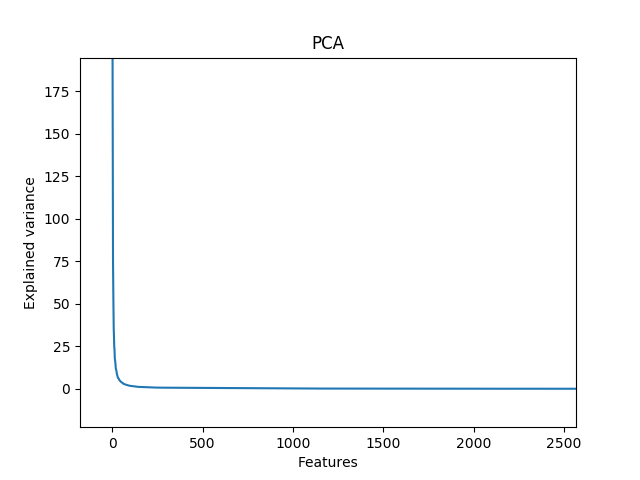
\includegraphics[width=0.8\textwidth]{Images/pca_var.png}
  \caption{Plot of explained variances of features}
\end{figure}

\begin{figure}[H]
  \centering
  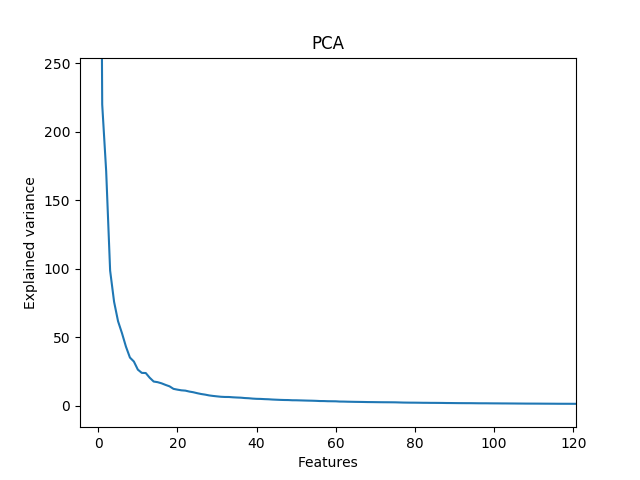
\includegraphics[width=0.8\textwidth]{Images/pca_var_zoom.png}
  \caption{Plot of explained variances of features(a closer look)}
\end{figure}

\subsection{Clustering}
Clustering is the task of dividing the population or data points into a number of groups such that data points in the same groups are more similar to other data points in the same group than those in other groups. A cluster is therefore a collection of objects which are “similar” between them and are “dissimilar” to the objects belonging to other clusters. Hence, clustering is a way of studying the underlying distribution for classification.\\

\textbf{DBSCAN}
Density-based spatial clustering of applications with noise (DBSCAN) is a data clustering algorithm which is density based: given a set of points in some space, it groups together points that are closely packed together (points with many nearby neighbors), marking as outliers points that lie alone in low density regions (whose nearest neighbors are too far away).

We tried Density Based Clustering on the dataset reduced to a feature space of 500 dimensions. Due to the large number of dimensions and instances, it was difficult loading the dataset into Weka. But the results obtained were poor as can be seen below :

\begin{figure}[H]
  \centering
  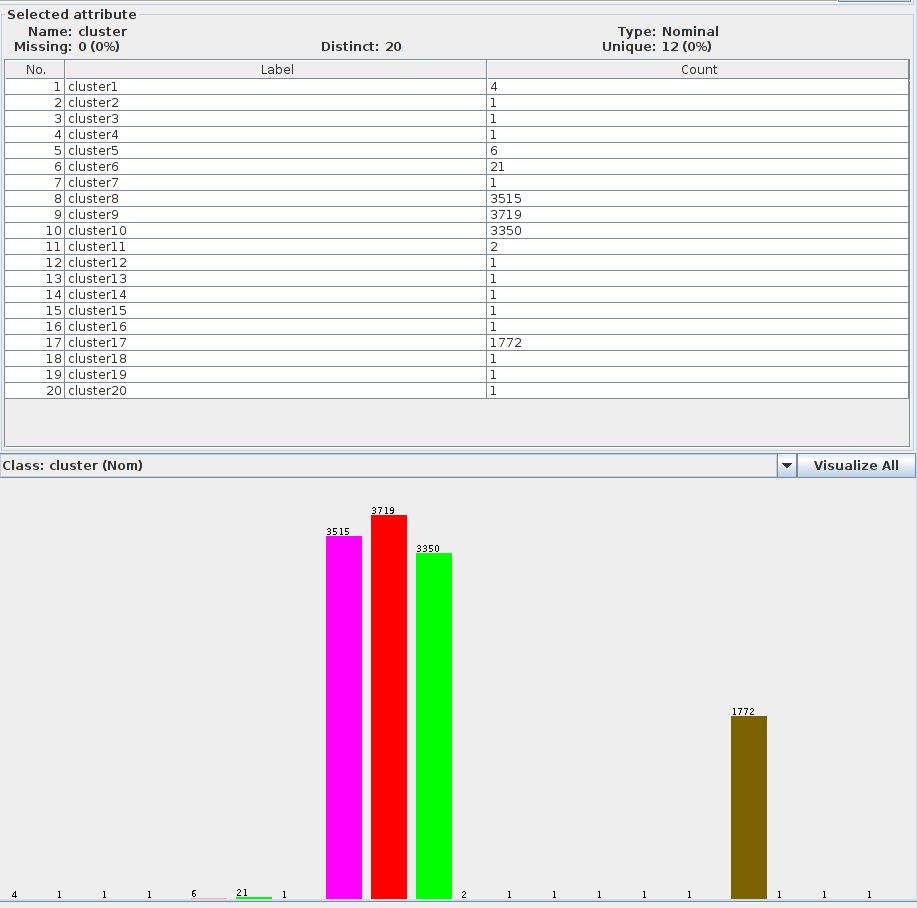
\includegraphics[width=0.8\textwidth]{Images/cluster_densitybased.png}
  \caption{Density Based Cluster : 500 features}
\end{figure}

\textbf{Kmeans: }It is a type of unsupervised learning, which aims to partition n observations into k clusters in which each observation belongs to the cluster with the nearest mean, serving as a prototype of the cluster.

We first tried k-means on the reduced feature space of 500 dimensions with k=10. The results obtained were as follows :
\begin{figure}[H]
  \centering
  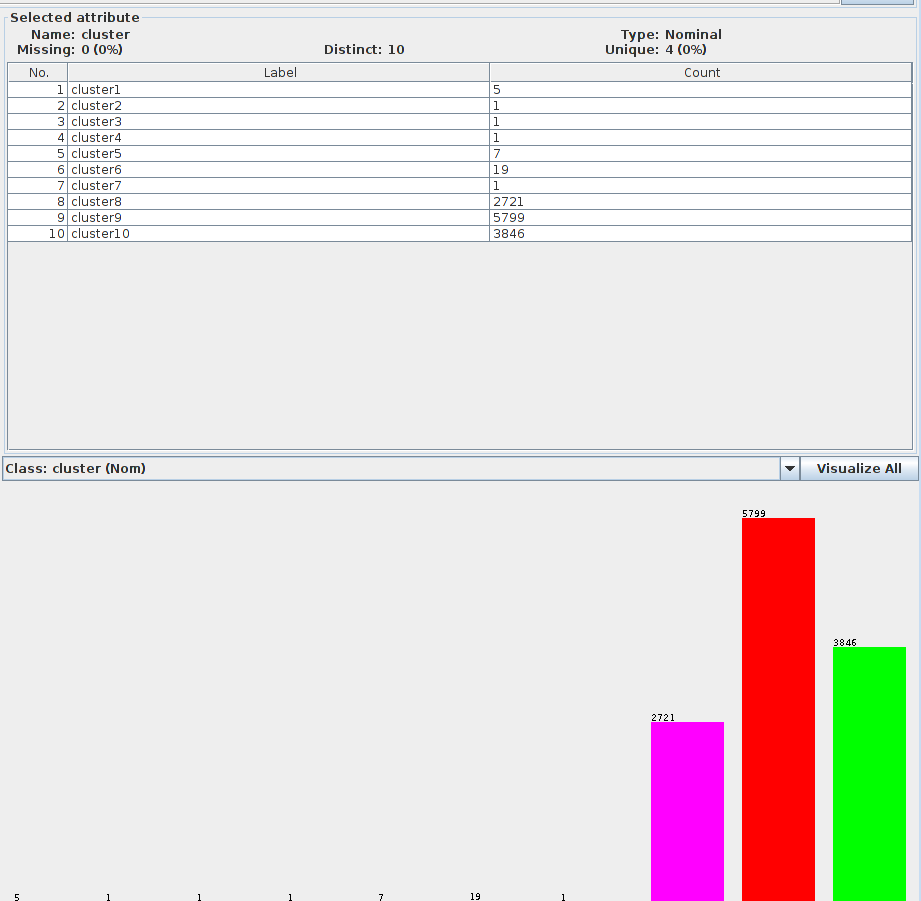
\includegraphics[width=0.8\textwidth]{Images/cluster_kmeans_10.png}
  \caption{K-Means (k=10) : 500 features}
\end{figure}

Hence, clustering wasn't considered in all the initial stages.\\

But towards the end, we tested K-means clustering on the original training dataset consisting of 2600 dimensions and 9501 instances. Loading the dataset onto Weka was very difficult and it failed multiple times. We were only able to load the full dataset once, and the results obtained have been depicted below :

\begin{figure}[H]
  \centering
  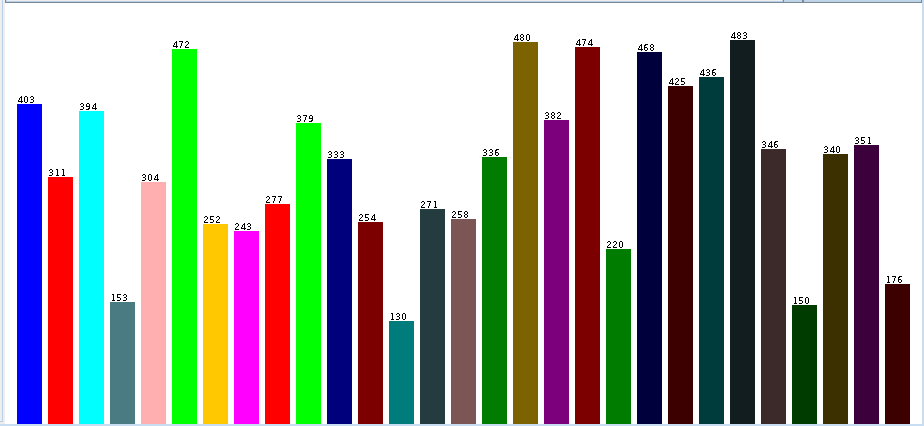
\includegraphics[width=0.8\textwidth]{Images/Labels_class_distribution.png}
  \caption{Class Labels : 2600 features}
\end{figure}

\begin{figure}[H]
  \centering
  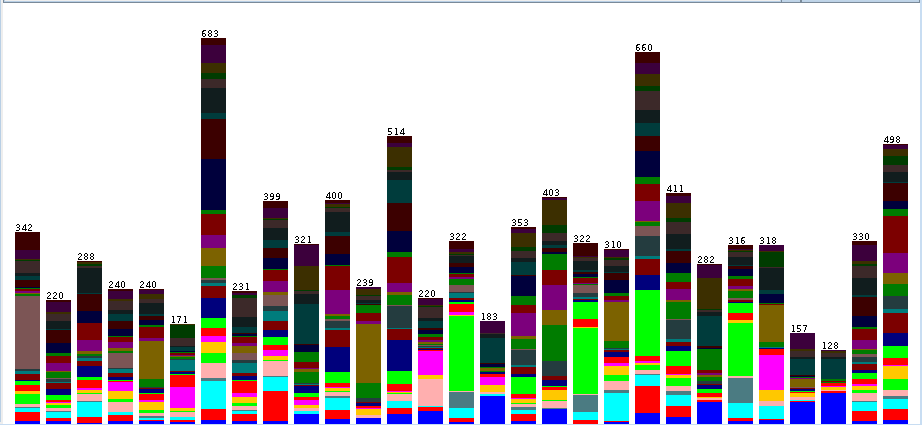
\includegraphics[width=0.8\textwidth]{Images/cluster1.png}
  \caption{K-Means (k=29) : 2600 features}
\end{figure}

The above image shows the fraction of cluster instances in each of the 29 clusters. It has been color-coded by the class label. Hence we can see that there are clusters that contain majority of a particular class instances. This gives us the inference that such classes are more easily identifiable when we run our classification algorithms. We can also see the class imbalances. Hence, we have to keep in mind that during classification, identification of the instances belonging to the minority class can be difficult.


%-------------------------------------------------------------------------------
% REFERENCES
%-------------------------------------------------------------------------------

\newpage
\section{Implemented Algorithms}

\subsection{Neural Networks}
A multilayer perceptron (MLP) is a class of feedforward artificial neural network. An MLP consists of at least three layers of nodes. Except for the input nodes, each node is a neuron that uses a nonlinear activation function. MLP utilizes a supervised learning technique called backpropagation for training. Its multiple layers and non-linear activation distinguish it from a linear perceptron. It can be utilised to distinguish data that is not linearly separable.\\

An MLP (or Artificial Neural Network - ANN) with a single hidden layer can be represented graphically as follows:

\begin{figure}[H]
  \centering
  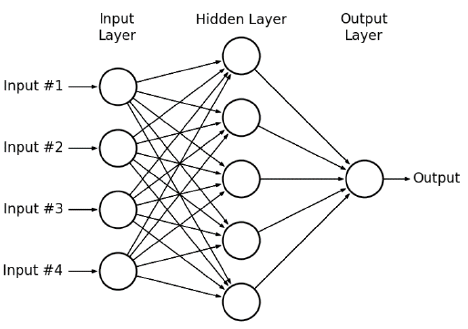
\includegraphics[width=0.8\textwidth]{Images/nn.png}
  \caption{Multilayer Layer Perceptron Network}
\end{figure}

The advantages of using Neutal Networs are as follows :
\begin{itemize}
    \item Adaptive learning: An ability to learn how to do tasks based on the data given for training or initial experience
    \item Self-Organisation: An ANN can create its own organisation or representation of the information it receives during learning time
    \item It has the ability to derive meaning from complicated or imprecise data, and can be used to extract patterns and detect trends that are too complex to be noticed by either humans or other computer techniques
\end{itemize}
\subsubsection{Procedure followed}
In addition to the hyperparameters of the neural net itself,there are a few other aspects that can be varied for this part. 
\begin{itemize}
    \item Out of all mentioned possibilities, what strategy was used to clean/impute the data.
    \begin{itemize}
        \item Median Imputation: did not work well(variance in these features drop significantly)
        \item Feature removal: The first five hundred features were thrown away. This is what gave the best results.
    \end{itemize}

    \item The are a large number of features in the data. What feature reduction/selection technique was used on the data.
    \begin{itemize}
        \item LDA :This does not work well at all.(possibly because the data is skewed)
        \item Raw data (after imputation/removal) 
        \item PCA Helped reduce the features, and enabled us to be able to apply more complex and computationally intensive models, while providing us with results in a reasonably short time interval.
    \end{itemize}

    \item What if multiple neural nets were sensitive to different classes. How do we combine the models?
    \begin{itemize}
        \item Mode:  We analysed the classification reports for models that had high f-scores, preferably with a different trend in fscores over different classes. Finally, the mode of the predictions was calculated(and submitted). This is the equivalent of a hard margin voting classifier with equal class weights.
        \item Weka J48: In order to combine the models in a more complex manner , we need an algo that is able work with data that has only nominal features. The J48 seems to do this. The validation fscore was observed to be 0.37, but on submission, we were only able to achieve a score of 0.30. 
        
    \end{itemize}
   
\end{itemize}
\subsubsection{(a) Hyperparameters}
The following values are a small subset of the set of values we tried(these worked relatively better).

\begin{table}[H]
\label{T:equipos}
\begin{center}
\begin{tabular}{| c | c | c | c | c |}
\hline
\textbf{PCA features} & \multicolumn{3}{ c |}{\textbf{MLP layers }} & \textbf{Avg Fscore} \\ 
\cline{2-4}
\textbf{n$\_$features} & \textbf{ Layer1} & \textbf{Layer 2} & \textbf{Layer 3} & \textbf{F-measure}\\
\hline

1400 & 800 & 800 & 1400 & 0.31  \\ \hline
800 & 800 & 800 & 400 & 0.32 \\ \hline
400 & 900  & 500 & 300 & 0.34  \\ \hline
100 & 800 & 800 & 400 & 0.38  \\ \hline
100 & 800 & 1200 & 300 & 0.41  \\ \hline
60 & 800 & 1200 & 300 & 0.42  \\ \hline
30 & 800 & 1200 & 300 & 0.35 \\ \hline

\end{tabular}
\end{center}
\end{table}
 (NOTE: The results are obtained after doing a 5 fold cross validation and choosing  the best performing model for each set of parameters) \\\\
The rest of the hyperparameters of the MLP classifier were kept constant. Some  of the other important hyperparameters are as follows:\\\\
Activation='relu', Solver='adam', alpha=0.0005, batch-size='auto',learning-rate='adaptive'\\ learning-rate-init=0.0005, power-t=0.5, max-iter=15000, shufle=True, random-state=5, tol=0.0001, early-stopping=False,validation-fraction=0.1\\

\newpage
The classification report for the best 2 models have been shown below :\\

Cross$\_$val2, PCA$\_$comp:60MLP layers: 800,1200,300  

\begin{figure}[H]
  \centering
  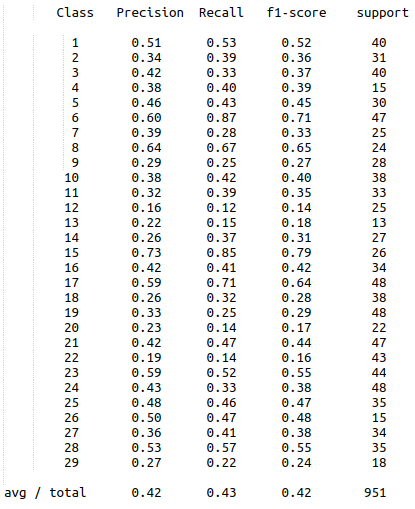
\includegraphics[width=0.8\textwidth]{Images/nn2.png}
  \caption{Classification Report}
\end{figure}

\newpage
Cross$\_$val1, PCA$\_$comp:80MLP layers: 1200,300,300   

\begin{figure}[H]
  \centering
  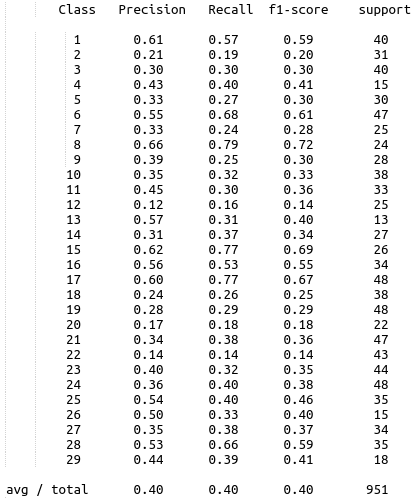
\includegraphics[width=0.8\textwidth]{Images/nn3.png}
  \caption{Classification Report}
\end{figure}


\newpage
\subsubsection{(b) Observation and Intuition}
From the table we notice a few things:
\begin{itemize}
    \item Increasing the number of features mostly does NOT increase the performance of the model.
    \item The The number of perceptrons in the first and second layer of the good models are much higher than the number of input. One possible explanation is that the first layer transforms the input into a "useful" set of features. Continuing on this logic, we tried increasing the number of inputs in the second layer as compared to the first. An f-score of 0.42 was achieved on the validation set.
    \item Decreasing the number of features to 30 does not work. So the knee point for optimal number of features must lie between 60 and 30.
\end{itemize}


\subsection{Random Forest}
Random forests is an ensemble learning method for classification, regression and other tasks, that operate by constructing a multitude of decision trees at training time and outputting the class that is the mode of the classes (classification) or mean prediction (regression) of the individual trees. It also reduces the chances of overfitting on the training data. The classifier creates the set of decision trees from randomly selected subset of training set (bagging).\\

The test labels were predicted by using two methods :
\begin{itemize}
    \item Taking the mode of the result of 5-fold cross-validation, ie, assigning the class predicted by majority of the folds.
    \item Summing up the class probabilities in each of the 5 folds for the predicted test labels and assigning it to the class having highest probability
\end{itemize}

This classifier was chosen over a single decision tree to counter overfitting and also get a more confident result as it is based on bagging and the result is given by an estimation from the predictions of all the estimators.\\

The classifier was tested using different sets of parameters. Two approaches were done :

\subsubsection{Reduced feature space}
Random forest was tested on the reduced feature space consisting of PCA reduced 500 features. Some of the best results obtained are as follows :\\


n$\_$estimators=2000, max$\_$depth=25, criterion='gini', min$\_$samples$\_$split=2, min$\_$samples$\_$leaf=1, n$\_$jobs=-1, verbose=1

\begin{figure}[H]
  \centering
  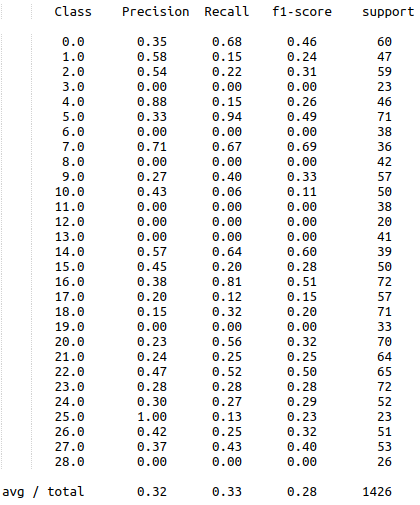
\includegraphics[width=0.7\textwidth]{Images/rf1.png}
  \caption{Random Forest : Classificatiion Report}
\end{figure}

\newpage
n$\_$estimators=1750, max$\_$depth=25, criterion='gini', min$\_$samples$\_$split=2, min$\_$samples$\_$leaf=1, n$\_$jobs=-1, verbose=1
\begin{figure}[H]
  \centering
  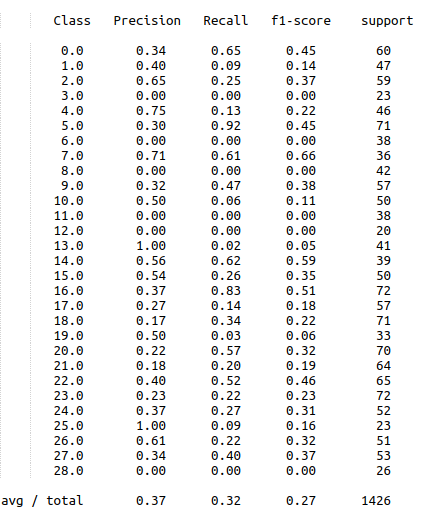
\includegraphics[width=0.7\textwidth]{Images/rf2.png}
  \caption{Random Forest : Classificatiion Report}
\end{figure}

\newpage
Some of the other good results obtained are as follows :
\begin{table}[H]
\label{T:equipos}
\begin{center}
\begin{tabular}{| c | c | c | c | c | c |}
\hline
\multicolumn{3}{| c |}{\textbf{Main Parameters}} & \multicolumn{3}{ c |}{\textbf{Average Estimates}} \\ 
\cline{1-6}
\textbf{n$\_$estimators} & \textbf{ max$\_$depth} & \textbf{criterion} & \textbf{Precision} & \textbf{Recall} & \textbf{F-measure}\\
\hline

3000 & 25  & Entropy & 0.28 & 0.29 & 0.24  \\ \hline
3000 & None & Entropy & 0.33 & 0.29 & 0.25 \\ \hline
\multicolumn{6}{| c |}{Balanced Subsample} \\ \hline
3000 & None  & Gini & 0.31 & 0.30 & 0.25  \\ \hline
6000 & None  & Gini & 0.35 & 0.30 & 0.25  \\ \hline
6000 & 15  & Gini & 0.30 & 0.28 & 0.25  \\ \hline
3000 & None  & Entropy & 0.30 & 0.29 & 0.24  \\ \hline
6000 & None  & Entropy & 0.40 & 0.29 & 0.24  \\ \hline
6000 & 60  & Entropy & 0.37 & 0.32 & 0.27  \\ \hline

\end{tabular}
\end{center}
\end{table}


The parameters other than the ones specified that have been used are :\\

 min$\_$weight$\_$fraction$\_$leaf=0.0, max$\_$features='auto', max$\_$leaf$\_$nodes=None, 
 
 min$\_$impurity$\_$decrease=0.0, min$\_$impurity$\_$split=None, bootstrap=True, oob$\_$score=False, random$\_$state=None, warm$\_$start=False
 
 
\newpage
\subsubsection{Imputed original feature space}
As the computation time for the algorithm was lesser compared to the other tested classifiers, we decided tot test Random forest with 2600 features per instance. The best 2 results obtained are as follows :\\

n$\_$estimators=2000, max$\_$depth=25, criterion='gini', min$\_$samples$\_$split=2, min$\_$samples$\_$leaf=1, n$\_$jobs=-1, verbose=1
\begin{figure}[H]
  \centering
  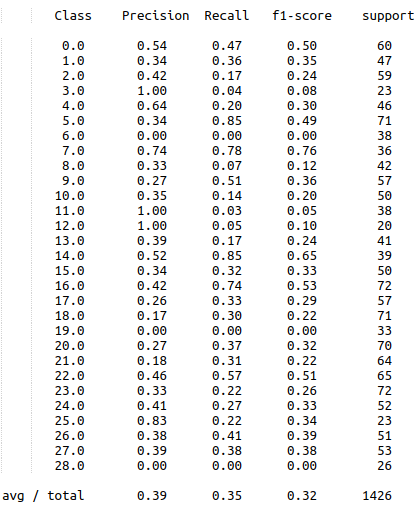
\includegraphics[width=0.7\textwidth]{Images/rf3.png}
  \caption{Random Forest : Classificatiion Report}
\end{figure}

\newpage
n$\_$estimators=1750, max$\_$depth=25, criterion='gini', min$\_$samples$\_$split=2, min$\_$samples$\_$leaf=1, n$\_$jobs=-1, verbose=1
\begin{figure}[H]
  \centering
  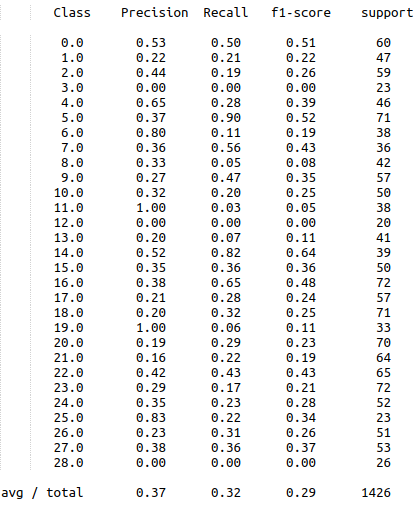
\includegraphics[width=0.7\textwidth]{Images/rf4.png}
  \caption{Random Forest : Classificatiion Report}
\end{figure}

The parameters other than the ones specified that have been used are :\\

 min$\_$weight$\_$fraction$\_$leaf=0.0, max$\_$features='auto', max$\_$leaf$\_$nodes=None, 
 
 min$\_$impurity$\_$decrease=0.0, min$\_$impurity$\_$split=None, bootstrap=True, oob$\_$score=False, random$\_$state=None, warm$\_$start=False

\newpage
\subsection{Adaboost}
An AdaBoost classifier begins by fitting a classifier on the original dataset and then fits additional copies of the classifier on the same dataset but where the weights of incorrectly classified instances are adjusted such that subsequent classifiers focus more on difficult cases. We tested the classifier using DecisionTreeClassifier. But the results obtained were poor. \\

The computation time of the algorithm was also very high, on a dataset with 500 features and 9501 instances and 5-fold cross-validation. The code, depending on the set of parameters took upto one full day to run.
The classifier was evaluated for various values of parameters :\\

DecisionTreeClassifier(max$\_$depth=3), n$\_$estimators=700, learning$\_$rate=0.1
\begin{figure}[H]
  \centering
  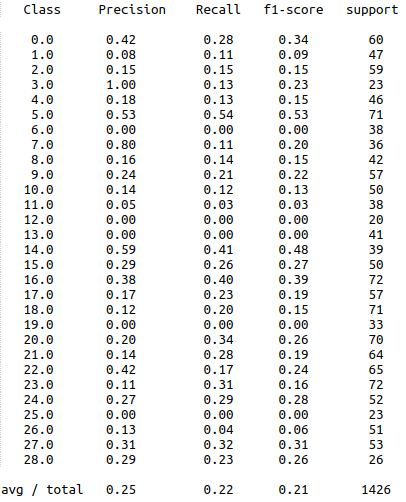
\includegraphics[width=0.7\textwidth]{ab.png}
  \caption{Adaboost Classificatiion Report}
\end{figure}

The test labels were predicted by using two methods :
\begin{itemize}
    \item Taking the mode of the result of 5-fold cross-validation, ie, assigning the class predicted by majority of the folds.
    \item Summing up the class probabilities in each of the 5 folds for the predicted test labels and assigning it to the class having highest probability
\end{itemize}

Using the probabilities and DecisionTreeClassifier(max$\_$depth=3), n$\_$estimators=800, learning$\_$rate=0.2
\begin{figure}[H]
  \centering
  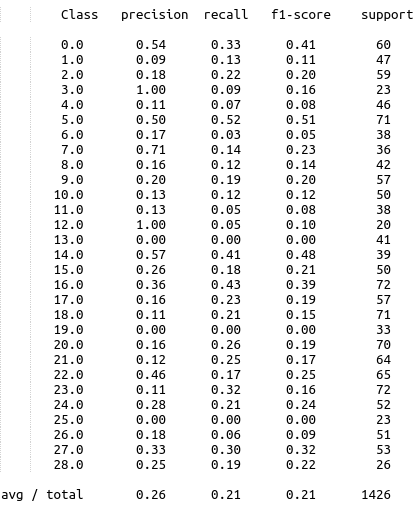
\includegraphics[width=0.7\textwidth]{Images/ab2.png}
  \caption{Adaboost Classificatiion Report}
\end{figure}

These are two of the best results obtained using the above classifier with a variety of parameters. Hence, this classifier was avoided during ensembling.

\newpage

Reasons why Decision tree was chosen as the classifier for boosting :
\begin{itemize}
    \item Theys are non-linear (Boosting with linear models doesn't usually work well)
    \item They are reasonably fast to train and classify
    \item By changing the depth, we have a simple and easy control over the bias/variance trade off\\\\
\end{itemize}

Reasons as to why Adaboost might have failed :
\begin{itemize}
    \item The noise level in the data: AdaBoost is particularly prone to overfitting on noisy datasets
    \item The dimensionality of the data: We know that generally, we experience overfitting more in high dimensional spaces, and AdaBoost can also suffer in that respect, as it is simply a linear combination of classifiers which themselves suffer from the problem
    \item Multi-label Classification: It is not an inherently multiclass classifier in sklearn\\\\
\end{itemize}

\subsection{Gradient Boost}
Gradient boosting is a machine learning technique for regression and classification problems, which produces a prediction model in the form of an ensemble of weak prediction models, typically decision trees. It builds the model in a stage-wise fashion like other boosting methods do, and it generalizes them by allowing optimization of an arbitrary differentiable loss function.\\

We worked a lot using gradient boosting with differnt sets of parameters. It was giving us better results than Adaboost and the performance on the cross-validation sets were upto what was obtained using Random Forests. The dataset used was the feature reduced dataset (PCA) comprising of 500 dimensions\\

\newpage
The test labels were predicted by using two methods :
\begin{itemize}
    \item Taking the mode of the result of 5-fold cross-validation, ie, assigning the class predicted by majority of the folds.
    \item Summing up the class probabilities in each of the 5 folds for the predicted test labels and assigning it to the class having highest probability
\end{itemize}

\begin{figure}[H]
  \centering
  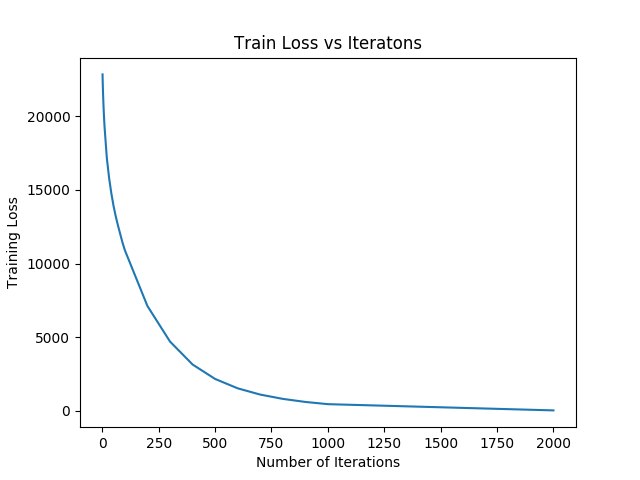
\includegraphics[width=0.7\textwidth]{Images/train_loss_gb.png}
  \caption{Training Loss}
\end{figure}

\newpage
The three best classifiers obtained among the lot :\\

n$\_$estimators=1500, learning$\_$rate=0.1, max$\_$depth=2, random$\_$state=0, verbose=1
\begin{figure}[H]
  \centering
  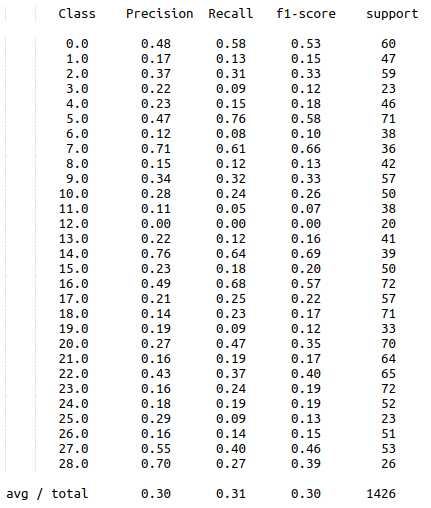
\includegraphics[width=0.7\textwidth]{Images/gb1.png}
  \caption{Gradient Boosting: Classification Report}
\end{figure}

\newpage
n$\_$estimators=2000, learning$\_$rate=0.15, max$\_$depth=2, random$\_$state=0, verbose=1
\begin{figure}[H]
  \centering
  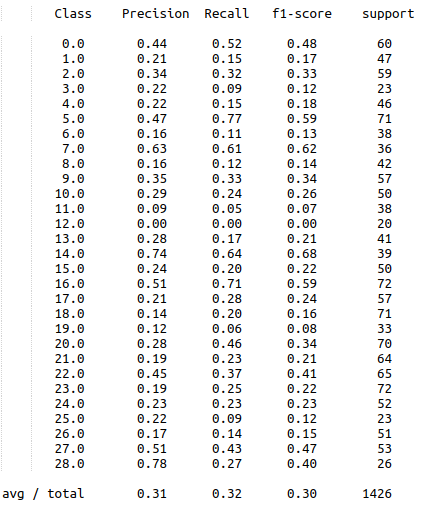
\includegraphics[width=0.7\textwidth]{Images/gb2.png}
  \caption{Gradient Boosting: Classification Report}
\end{figure}

\newpage
n$\_$estimators=2000, learning$\_$rate=0.05, max$\_$depth=2, random$\_$state=0, verbose=1
\begin{figure}[H]
  \centering
  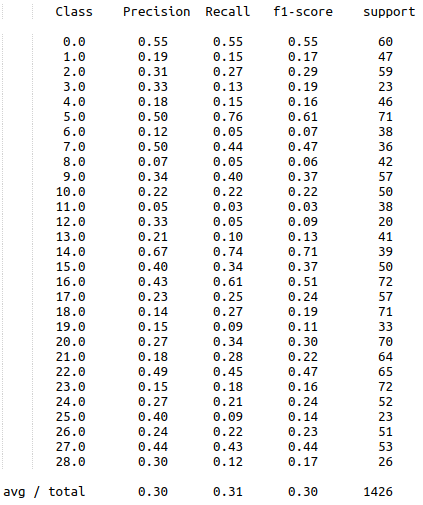
\includegraphics[width=0.7\textwidth]{Images/gb3.png}
  \caption{Gradient Boosting: Classification Report}
\end{figure}

\newpage
Some of the other results obtained are as follows :
\begin{table}[H]
\label{T:equipos}
\begin{center}
\begin{tabular}{| c | c | c | c | c | c |}
\hline
\multicolumn{3}{| c |}{\textbf{Main Parameters}} & \multicolumn{3}{ c |}{\textbf{Average Estimates}} \\ 
\cline{1-6}
\textbf{n$\_$estimators} & \textbf{ max$\_$depth} & \textbf{learning rate} & \textbf{Precision} & \textbf{Recall} & \textbf{F-measure}\\
\hline

1000 & 1  & 0.5 & 0.21 & 0.23 & 0.21  \\ \hline
2000 & 1  & 0.5 & 0.21 & 0.23 & 0.21  \\ \hline
3000 & 1 & 0.25 & 0.26 & 0.26 & 0.25 \\ \hline
4000 & 1  & 0.15 & 0.27 & 0.27 & 0.26  \\ \hline
6000 & 1  & 0.15 & 0.26 & 0.27 & 0.26  \\ \hline
6000 & 3  & 0.5 & 0.19 & 0.20 & 0.19  \\ \hline
9000 & 1  & 0.2 & 0.26 & 0.26 & 0.25  \\ \hline
2000 & 3  & 0.1 & 0.27 & 0.30 & 0.28  \\ \hline
4000 & 3  & 0.09 & 0.28 & 0.30 & 0.29  \\ \hline
2000 & 3  & 0.05 & 0.30 & 0.31 & 0.29  \\ \hline

\end{tabular}
\end{center}
\end{table}

Observed Disadvantages :
\begin{itemize}
    \item The code took over a day to run, probably because of the fact that trees are built sequentially and the data has high dimensionality (500 dimensions - PCA reduced)
    \item There are 3 main parameters to train : learning rate, depth of tree and number of trees. Now each of these parameters should be tuned to get a good fit. This was difficult to achieve keeping in mind the time constraint and the available resources and the fact that the classifier is prone to overfitting
\end{itemize}

\subsection{Naive Bayes}
The Naive Bayes Classifier technique is based on the Bayesian theorem and is suitable when the dimensionality of the inputs is high. The different naive Bayes classifiers differ mainly by the assumptions they make regarding the distribution of P(${x_{i}} \mid y)$.


\subsubsection{Gaussian}
Here we are dealing with continuous data, so we assume that the continuous values associated with each class are distributed according to a Gaussian distribution. For the training data containing a continuous attribute x, we first segment the data by the class, and then compute the mean and variance of x in each class.\\

The sklearn Naive Bayes Packages was tested on the features for the reduced feature space (500 dimensions) (by using PCA) and the following results were observed :

\begin{figure}[H]
  \centering
  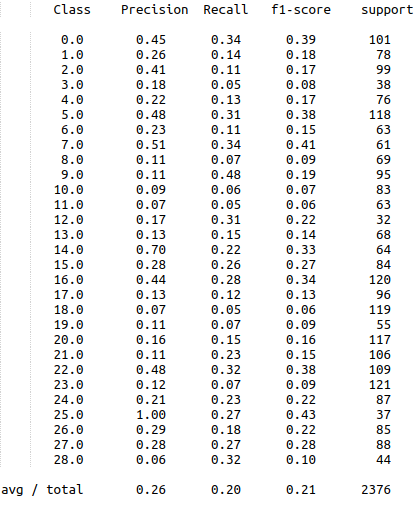
\includegraphics[width=0.7\textwidth]{Images/nb_g.png}
  \caption{Naive Bayes: Classification Report}
\end{figure}

Due to the poor results obtained, this further work was not done on the classifier.\\
One possible reason why naive bayes does'nt work well: It's basic assumption on strong feature independence must have been violated. Possibly there is still some dependencies among the features that we were not able to eliminate.\\


\subsection{SVM}
Support Vector Machines (SVMs) are supervised learning models with associated learning algorithms that analyze data used for classification and regression. In addition to performing linear classification, SVMs can efficiently perform a non-linear classification using what is called the kernel trick, implicitly mapping their inputs into high-dimensional feature spaces.

\subsubsection{Sigmoid Kernel}
The sigmoid kernel function is of the form :
$$tanh(\gamma<x,x'> + r)$$

But our input dimension is 2600 with 9501 instances and hence, even after running the algorithm for more than 3 days, convergence was not obtained and hence the algorithm was discarded and not worked on further.

\subsubsection{Gaussian Kernel}
The Gaussian kernel function is of the form :
$$\exp(-\gamma||x-x'||^{2})$$

The code ran for a long time, and did'nt seem to be close to finishing any time soon.\\

Probable reason:SVM when used for multiclass classification uses either one of 'ovr'-one-vs-rest or 'ovo'- one-vs-one. When running for a problem  with 29 classes, the number of combinations required in ovo is too much, and the class imbalance in case of ovr is too high. This lead us to rule out SVM as a feasible method of solving the given problem.


\subsection{XGBoost}
XGBoost is short for “Extreme Gradient Boosting”, as it is an optimized distributed gradient boosting library. It is an open-source software library which provides the gradient boosting framework.

Advantages of XGBoost over gradient boosted trees :
\begin{itemize}
    \item Parallel Computing: It is enabled with parallel processing (using OpenMP); i.e., when we run xgboost, by default, it would use all the cores of our laptop.
    \item Regularization: GBM has no provision for regularization. Regularization is a technique used to avoid overfitting in linear and tree-based models.
    \item Tree Pruning: Unlike GBM, where tree pruning stops once a negative loss is encountered, XGBoost grows the tree upto max$\_$depth and then prune backward until the improvement in loss function is below a threshold.
\end{itemize}

XGBoost was implemented on the feature reduced dataset comprising of 500 PCA reduced features. Some of the best results obtained are as follows :

n$\_$estimators=1000
\begin{figure}[H]
  \centering
  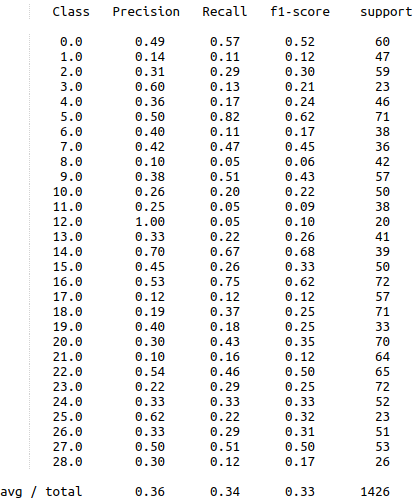
\includegraphics[width=0.7\textwidth]{Images/xgb1.png}
  \caption{XGBoost: Classification Report}
\end{figure}

\newpage
n$\_$estimators=1500
\begin{figure}[H]
  \centering
  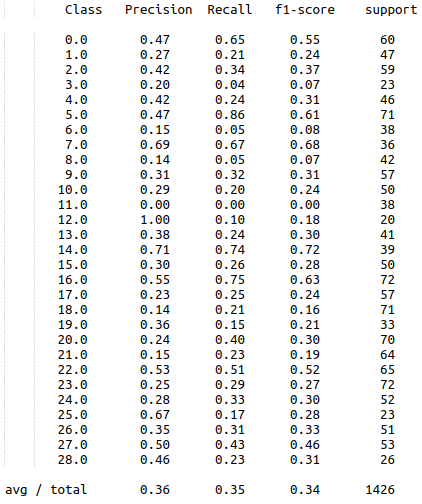
\includegraphics[width=0.7\textwidth]{Images/xgb2.png}
  \caption{XGBoost: Classification Report}
\end{figure}

\newpage
n$\_$estimators=2000
\begin{figure}[H]
  \centering
  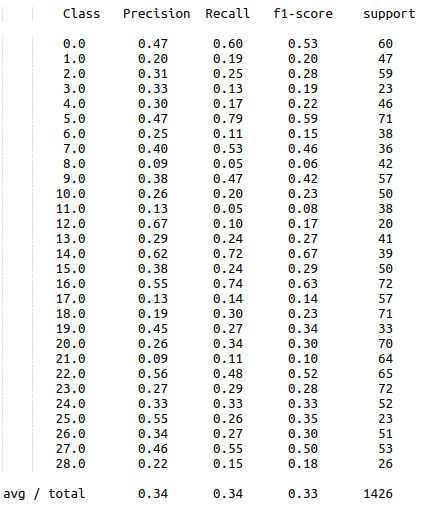
\includegraphics[width=0.7\textwidth]{Images/xgb3.png}
  \caption{XGBoost: Classification Report}
\end{figure}

Among the classifiers, other than MLP that was used, this gave the highest results and hence, it was considered during ensembling.

\newpage
\subsection{Voting Classifier}
The idea behind the VotingClassifier is to combine conceptually different machine learning classifiers and use a majority vote or the average predicted probabilities (soft vote) to predict the class labels. Such a classifier can be useful for a set of equally well performing model in order to balance out their individual weaknesses.\\

We have used soft voting, as it returns the class label as argmax of the sum of predicted probabilities. The saved best models (using pickle) of Random Forest, Gradient Boosting and XGB Boosting were used for building the Voting classifier. The feature reduced dataset comprising of 500 dimensions were used during the computation. The computation proved to be very expensive and took more than 2 days to reach convergence when implemented using 5-fold cross-validation.\\

The results obtained are as follows :
\begin{itemize}
    \item XGBoost : n$\_$estimators=1500
    \item Gradient Boosting : n$\_$estimators=1500, learning$\_$rate=0.1, max$\_$depth=2, random$\_$state=0, verbose=1
    \item Random Forest : n$\_$estimators=2000, max$\_$depth=25, criterion='gini', min$\_$samples$\_$split=2, min$\_$samples$\_$leaf=1, n$\_$jobs=-1, verbose=1
\end{itemize}

\begin{figure}[H]
  \centering
  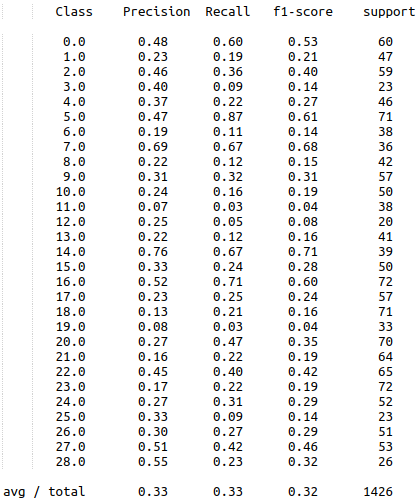
\includegraphics[width=0.8\textwidth]{Images/vote.png}
  \caption{Voting Classifier: Classification Report}
\end{figure}

\newpage
\section{Our Insights about the Dataset }
Here are some points we have concluded about the data (both major and minor)
\begin{itemize}
    \item From our experience with the data, based on observed patterns of missing features and variance patterns, it looks like the data was artificially generated.
    \item The data has already been scaled and normalised. But even then, the number of ones varies from 3-9 percent of each feature . Class 7 seems to have the highest number of features per data point taking the value 1. This could been caused by some kind of overflow/threshold.
    \item We also feel that the number of important features in the dataset are relatively low in comparison to the the number of features given. This conclusion is supported by our observations on PCA variances and trends in neural net result.
    \item The data generation could have been achieved by generating a couple of features, and performing some complex transformations on them and appending the results to the dataset as new features. 
    \item Also, when visualising the features, one can directly conclude that linear models are not feasible, as histogram plots of features show varying percentages of each classes data points in every range. Also, the data distribution within most of the features is skewed.
\end{itemize}


\newpage  
\section{Final Model}

Till now, we have presented and explained all the models that we tried out. Here is a description of the final model that we have submitted:
\begin{itemize}
    \item First the data was cleaned. That is we threw away the first 500 features.
    \item Next we performed PCA and extracted some features. Mostly in the set of {50,60,80,100,200}
    \item Then we passed the extracted features to a neural net. We made sure that the first layer of the neural net had a much larger number of features than the number of inputs.
    \item Finally, we analysed the classification reports of multiple models and put together models that collectively had a decent fscore in all the classes. The mode of the models at each data point was computed.
    \item In order to make our model more robust, we combined many models with fscores ranging from 0.38 to 0.42, where some of their individual class fscores were higher than those in other models 
    \item We then submitted our result :)
\end{itemize}

%-------------------------------------------------------------------------------
% REFERENCES
%-------------------------------------------------------------------------------
\newpage
\section*{References}
\addcontentsline{toc}{section}{References}

\begin{sloppypar}

\url{http://scikit-learn.org/stable/modules/generated/sklearn.ensemble.VotingClassifier.html}
\newline
\noindent


\url{http://scikit-learn.org/stable/modules/ensemble.html#voting-classifier}
\newline
\noindent


 \url{https://cran.r-project.org/web/packages/xgboost/xgboost.pdf}
\newline
\noindent


 \url{http://scikit-learn.org/stable/modules/svm.html}
\newline
\noindent


 \url{https://www.youtube.com/watch?v=1SxPbhaK_uc&list=PL1xHD4vteKYVpaIiy295pg6_SY5qznc77&index=68}
\newline
\noindent


 \url{http://scikit-learn.org/stable/modules/generated/sklearn.ensemble.AdaBoostClassifier.html}
\newline
\noindent


 \url{http://scikit-learn.org/stable/modules/multiclass.html}
\newline
\noindent

 \url{http://scikit-learn.org/stable/modules/generated/sklearn.ensemble.ExtraTreesClassifier.html#sklearn.ensemble.ExtraTreesClassifier}
\newline
\noindent


\url{http://scikit-learn.org/stable/modules/generated/sklearn.naive_bayes.GaussianNB.html#sklearn.naive_bayes.GaussianNB}
\newline
\noindent


 \url{http://scikit-learn.org/stable/modules/generated/sklearn.neighbors.KNeighborsClassifier.html#sklearn.neighbors.KNeighborsClassifier}
\newline
\noindent


 \url{http://scikit-learn.org/stable/modules/generated/sklearn.discriminant_analysis.LinearDiscriminantAnalysis.html#sklearn.discriminant_analysis.LinearDiscriminantAnalysis}
\newline
\noindent


 \url{http://scikit-learn.org/stable/modules/generated/sklearn.neural_network.MLPClassifier.html#sklearn.neural_network.MLPClassifier}
\newline
\noindent


 \url{http://scikit-learn.org/stable/modules/generated/sklearn.ensemble.RandomForestClassifier.html#sklearn.ensemble.RandomForestClassifier}
\newline
\noindent


 \url{http://scikit-learn.org/stable/modules/generated/sklearn.svm.SVC.html#sklearn.svm.SVC}
\newline
\noindent


 \url{http://scikit-learn.org/stable/modules/generated/sklearn.ensemble.GradientBoostingClassifier.html#sklearn.ensemble.GradientBoostingClassifier}

\end{sloppypar}



\end{document}

%-------------------------------------------------------------------------------
% SNIPPETS
%-------------------------------------------------------------------------------

%\begin{figure}[!ht]
%	\centering
%	\includegraphics[width=0.8\textwidth]{file_name}
%	\caption{}
%	\centering
%	\label{label:file_name}
%\end{figure}

%\begin{figure}[!ht]
%	\centering
%	\includegraphics[width=0.8\textwidth]{graph}
%	\caption{Blood pressure ranges and associated level of hypertension (American Heart Association, 2013).}
%	\centering
%	\label{label:graph}
%\end{figure}

%\begin{wrapfigure}{r}{0.30\textwidth}
%	\vspace{-40pt}
%	\begin{center}
%		\includegraphics[width=0.29\textwidth]{file_name}
%	\end{center}
%	\vspace{-20pt}
%	\caption{}
%	\label{label:file_name}
%\end{wrapfigure}

%\begin{wrapfigure}{r}{0.45\textwidth}
%	\begin{center}
%		\includegraphics[width=0.29\textwidth]{manometer}
%	\end{center}
%	\caption{Aneroid sphygmomanometer with stethoscope (Medicalexpo, 2012).}
%	\label{label:manometer}
%\end{wrapfigure}

%\begin{table}[!ht]\footnotesize
%	\centering
%	\begin{tabular}{cccccc}
%	\toprule
%	\multicolumn{2}{c} {Pearson's correlation test} & \multicolumn{4}{c} {Independent t-test} \\
%	\midrule	
%	\multicolumn{2}{c} {Gender} & \multicolumn{2}{c} {Activity level} & \multicolumn{2}{c} {Gender} \\
%	\midrule
%	Males & Females & 1st level & 6th level & Males & Females \\
%	\midrule
%	\multicolumn{2}{c} {BMI vs. SP} & \multicolumn{2}{c} {Systolic pressure} & \multicolumn{2}{c} {Systolic Pressure} \\
%	\multicolumn{2}{c} {BMI vs. DP} & \multicolumn{2}{c} {Diastolic pressure} & \multicolumn{2}{c} {Diastolic pressure} \\
%	\multicolumn{2}{c} {BMI vs. MAP} & \multicolumn{2}{c} {MAP} & \multicolumn{2}{c} {MAP} \\
%	\multicolumn{2}{c} {W:H ratio vs. SP} & \multicolumn{2}{c} {BMI} & \multicolumn{2}{c} {BMI} \\
%	\multicolumn{2}{c} {W:H ratio vs. DP} & \multicolumn{2}{c} {W:H ratio} & \multicolumn{2}{c} {W:H ratio} \\
%	\multicolumn{2}{c} {W:H ratio vs. MAP} & \multicolumn{2}{c} {\% Body fat} & \multicolumn{2}{c} {\% Body fat} \\
%	\multicolumn{2}{c} {} & \multicolumn{2}{c} {Height} & \multicolumn{2}{c} {Height} \\
%	\multicolumn{2}{c} {} & \multicolumn{2}{c} {Weight} & \multicolumn{2}{c} {Weight} \\
%	\multicolumn{2}{c} {} & \multicolumn{2}{c} {Heart rate} & \multicolumn{2}{c} {Heart rate} \\
%	\bottomrule
%	\end{tabular}
%	\caption{Parameters that were analysed and related statistical test performed for current study. BMI - body mass index; SP - systolic pressure; DP - diastolic pressure; MAP - mean arterial pressure; W:H ratio - waist to hip ratio.}
%	\label{label:tests}
%\end{table}